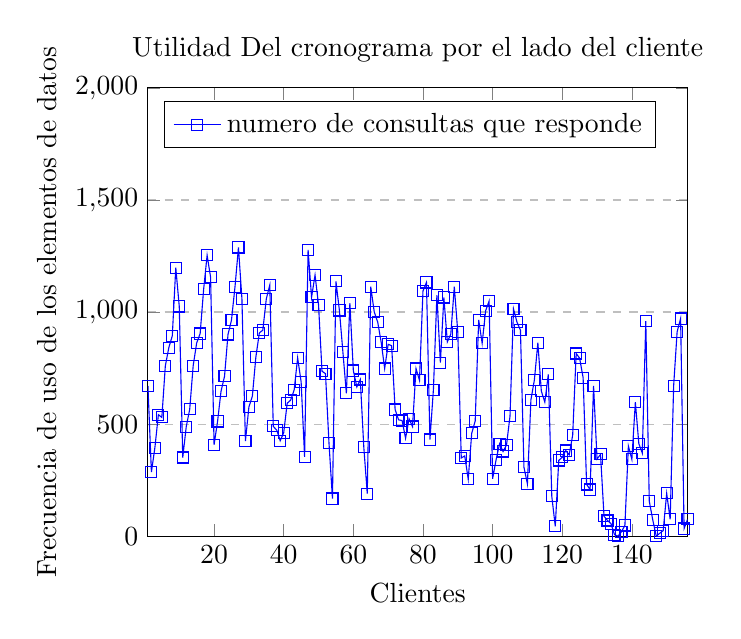
\begin{tikzpicture}
\begin{axis}[
    title={Utilidad Del cronograma por el lado del cliente},
    xlabel={Clientes},
    ylabel={Frecuencia de uso de los elementos de datos},
    xmin=1, xmax=156,
    ymin=0, ymax=2000,
    xtick={},
    ytick={},
    legend pos=north west,
    ymajorgrids=true,
    grid style=dashed,
]

\addplot[
    color=blue,
    mark=square,
    ]
    coordinates {
    %USO EXACTO
    (1,671)
(2,286)
(3,395)
(4,542)
(5,530)
(6,760)
(7,841)
(8,894)
(9,1198)
(10,1025)
(11,351)
(12,488)
(13,566)
(14,761)
(15,862)
(16,904)
(17,1101)
(18,1253)
(19,1155)
(20,408)
(21,512)
(22,647)
(23,713)
(24,900)
(25,964)
(26,1111)
(27,1288)
(28,1059)
(29,424)
(30,576)
(31,625)
(32,799)
(33,907)
(34,919)
(35,1059)
(36,1120)
(37,490)
(38,473)
(39,426)
(40,462)
(41,593)
(42,607)
(43,652)
(44,796)
(45,689)
(46,354)
(47,1277)
(48,1066)
(49,1165)
(50,1033)
(51,736)
(52,725)
(53,417)
(54,168)
(55,1137)
(56,1007)
(57,822)
(58,637)
(59,1040)
(60,739)
(61,666)
(62,699)
(63,398)
(64,190)
(65,1113)
(66,1001)
(67,955)
(68,865)
(69,748)
(70,856)
(71,850)
(72,565)
(73,519)
(74,516)
(75,437)
(76,524)
(77,489)
(78,748)
(79,695)
(80,1094)
(81,1132)
(82,431)
(83,654)
(84,1075)
(85,774)
(86,1065)
(87,867)
(88,902)
(89,1113)
(90,910)
(91,349)
(92,358)
(93,254)
(94,459)
(95,514)
(96,965)
(97,861)
(98,1006)
(99,1049)
(100,256)
(101,341)
(102,412)
(103,378)
(104,407)
(105,536)
(106,1014)
(107,955)
(108,919)
(109,308)
(110,233)
(111,608)
(112,697)
(113,863)
(114,647)
(115,598)
(116,722)
(117,178)
(118,44)
(119,338)
(120,352)
(121,382)
(122,363)
(123,451)
(124,815)
(125,794)
(126,707)
(127,231)
(128,208)
(129,670)
(130,344)
(131,365)
(132,89)
(133,70)
(134,56)
(135,7)
(136,0)
(137,20)
(138,48)
(139,402)
(140,343)
(141,598)
(142,413)
(143,371)
(144,959)
(145,156)
(146,73)
(147,0)
(148,13)
(149,25)
(150,191)
(151,75)
(152,671)
(153,912)
(154,971)
(155,34)
(156,75)
    };
    \legend{numero de consultas que responde}

\end{axis}
\end{tikzpicture}

